\documentclass[11pt, twocolumn]{jsarticle}
\usepackage[dvipdfmx,hiresbb]{graphicx}

\begin{document}

\title{音楽再生と時刻の関係}
\author{藤賀雄太}
\date{2012年12月10日}
\begin{abstract}
音楽再生における推薦システムに役立てることを目標として、音楽再生と時刻の関係を調べたものである。
ジャンルの関連性や、音楽のビート情報などの音楽自体の情報による音楽推薦システムでもなく、
ランダム再生でもない、
ユーザーの時刻に準拠した音楽推薦システムを提案する。
\end{abstract}
\maketitle
\tableofcontents


\section{イントロダクション}
\subsection{世の中の現状分析}
音楽記録メディアはデジタル化によって小型化が進み、携帯可能になった。(以後、モバイルプレイヤーと呼ぶ)
ウォークマンやiPodを代表とする再生専用機器は広く普及したが、
最近では、携帯電話と一体型になっているものも広く普及しており、音楽を再生できる機器を常に持ち歩くと言うことが一般的になった。
また、スピーカーではなく、ヘッドホンで聴く場合、自分だけ聴くことができるため、
例えば電車の中などの公共空間で聴くことや、学校の授業の合間の時間にすぐに取り出して聴けるようになった。
そのため、音楽を聴く場所と時間に制約がなくなり、
どんな時刻でも、どこにいても、好きな楽曲を聴くことができるようになった。

\subsection{現状分析から見えてくる問題点}
モバイルプレイヤーには、たくさんの楽曲を入れることができる便利さがある一方、
多くの楽曲の中から今聴きたい音楽を選択することは容易ではない。
そのため、モバイルプレイヤーには自動的に音楽を再生する機能が付いていることが多い。
今回の実験で使用したiTunesにもGeniusとシャッフルの2つの機能が付いている。
Geniusはジャンルをベースとした、音楽リコメンドで、現在最も広く使われている音楽推薦方式である。
シャッフル機能はユーザーがiTunesに入れている楽曲から無作為に音楽を選んで再生する。
なんでもよいからなんか聴きたいという場合に、自分の気持ちや状況とは無関係に選択されることで、
長時間マンネリすることなく聴くことができるため、1つの音楽推薦方式であると考ることもできる。
シャッフル機能は大変人気があり、本実験でのアンケートによると、半数以上の人がシャッフル機能を利用していた。
シャッフルは、アーティスト名や、ジャンル名などを入力することによって、
全ての楽曲から、特定の範囲にしぼった楽曲群の中で再生することもできるため、
選ぶことと、無作為に選ばれることを組み合わせて使うこともできる。
このように、無作為に選択する対象に対してユーザーの好みの情報を入力することによって、ユーザーが自分自身に対して推薦することができる。
しかし、ユーザーの聴きたい音楽を得るためには、ジャンル名のような音楽自体にタグづけられた情報とは限らない。
寝る前に聴くとか、テンション上げたいといったことがあってもその言葉を検索しても1曲も得られないであろう。
また、これらのユーザーの気分をユーザー自身が自分で入力することは容易ではない。
また、ユーザーが自分がどんな時間に音楽を聴いているのかを自覚していない場合もあるため、
システムがユーザーの操作履歴からユーザーがどんな時刻に何を聴いているのかを学習して、
ユーザーの状況を推測し、ユーザーはその推測された結果だけを聴くもしくは、評価することが適切である。

音楽を再生するときの状況には、さまざまな情報がある。
それは、好きな音楽のジャンルといった音楽それ自体の情報もあるが、
一方で、気分によって変えるといったように、
再生するその場の気分や、読書中だからといった状況によってなどの、
音楽それ自体の情報以外の、外的な情報によって適宜選ぶこともある。
それは、音楽を再生するときの条件が一様ではなく、絶えず変化する動的なものだからだ。
その気分といった不確定なものに、ある周期的なものを見つけることで、
気分に対して柔軟に変化するリコメンドがあれば、ユーザーは煩雑な選択の操作からも開放されるだけでなく、
無機質なランダム再生による気分との不一致から解放されることになるではないかと考えた。
また、そのことによって、ジャンルを中心とした音楽の好みによるリコメンドサービスの精度向上も期待できるのではないかと考えた。
例えば、朝の時間はクラシックを中心に聴くことをを好み、夜には、ジャズを中心に聴く人がいたとすると、
ジャンルだけの音楽の好みでみると、ジャズとクラシックを交互に再生するリコメンドとなってしまうことで、推薦の効果は小さい。
一方、ジャズのジャンルを選択してシャッフル機能を利用していたとして、それはジャズの中ではランダムに再生されるものの、
他のジャンルは再生されないので、単調になってしまう。
つまり、ジャンルによって音楽を選択する人であってすら、ジャンルだけの音楽リコメンドは、他のコンテキストの情報によって変化する場合は、
パフォーマンスが下がってしまうこともあるのだ。

\subsection{現状分析から見えてくるチャンス}
楽曲の音楽の情報自体にアクセスするのではなく、楽曲が再生される状況の関係性から楽曲を分析することができるのではないかと考えた。
リコメンドサービスにおいてはジャンルによって推薦するものが多いが、
ユーザーが考える音楽ジャンルと必ずしも一致しているとは限らないし、
ユーザーが自分の聴いているジャンルを把握しているとは限らない。
そこで、時刻という切り口で音楽再生の履歴情報を分析することで、
ユーザーが音楽を再生するときの、その時刻の情報によって、音楽を推薦できないかと考えた。

\subsection{特に注目する問題ひとつ(研究課題)}
\subsubsection{実験の背景}
音楽再生時のユーザー自身の状況から、音楽を推薦するために、
いくつかの要素を抽出して、予備的な音楽再生ソフトを自作して、
自分で使ってみたり、プレゼンやデモを通して第三者からもフィードバックをもらったりした。
それを踏まえて時刻に着目し、本研究にいたった。その背景をここで説明したい。
ここでは、簡単に以下に紹介する。
\begin{enumerate}
\item
場所

\subsubsection{Music Earth}

\begin{figure}[h]
\begin{center}
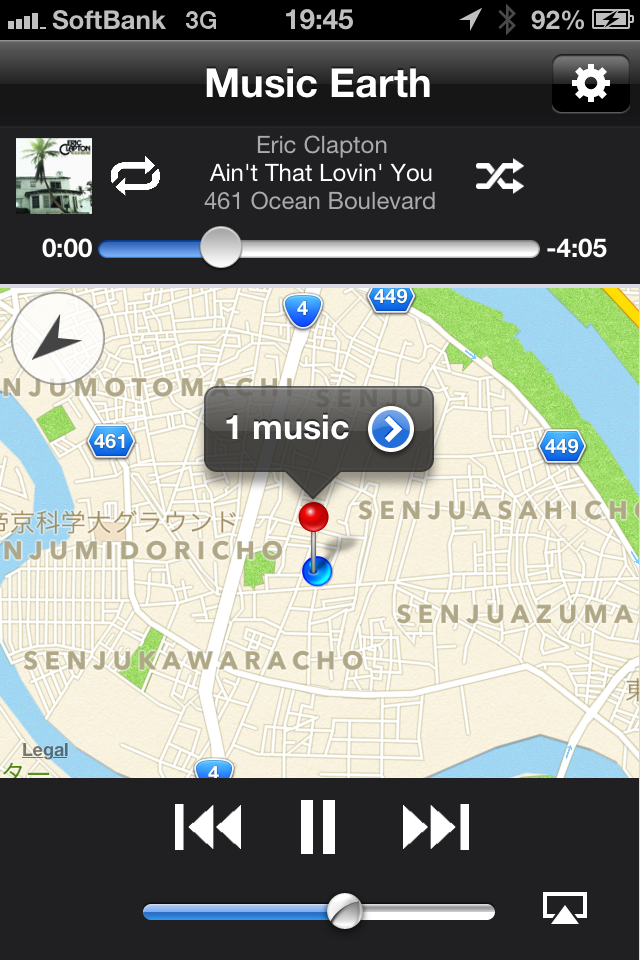
\includegraphics[width=5.866cm]{musicEarth.png}
\caption{Music Earthのインターフェース}
\label{musicEarth_interface}
\end{center}
\end{figure}

GPSを利用して音楽の履歴情報を地図にプロットしていくことで、地図全体が音楽のプレイリストとなり、
再生時の位置情報によって、以前その場所周辺で再生された楽曲の中からその場所に近ければ近いほど高確率で推薦される音楽再生アプリケーション。
iPhone用のアプリケーションで、iPhoneの音楽ライブラリと連携している。
音楽を聴いたら、地図上に聴いた位置情報と、聴いた楽曲を記録する。
地図から以前その場所で聴いた音楽を選択して聴くこともできる。
\subsubsection{Place Melody}

地図に聴きたい音楽を配置していき、自分がその場所に近づくと再生されるiPhone用アプリケーション。
選択しなければいけない音楽再生ではなく、場所から聞こえてくる音楽ということとをテーマに制作した。
電車に乗っていても音楽によって、目的地に到着したことを知ることができるなど、場所によって自分の音楽体験をデザインすることができる。

\begin{figure}[h]
\begin{center}
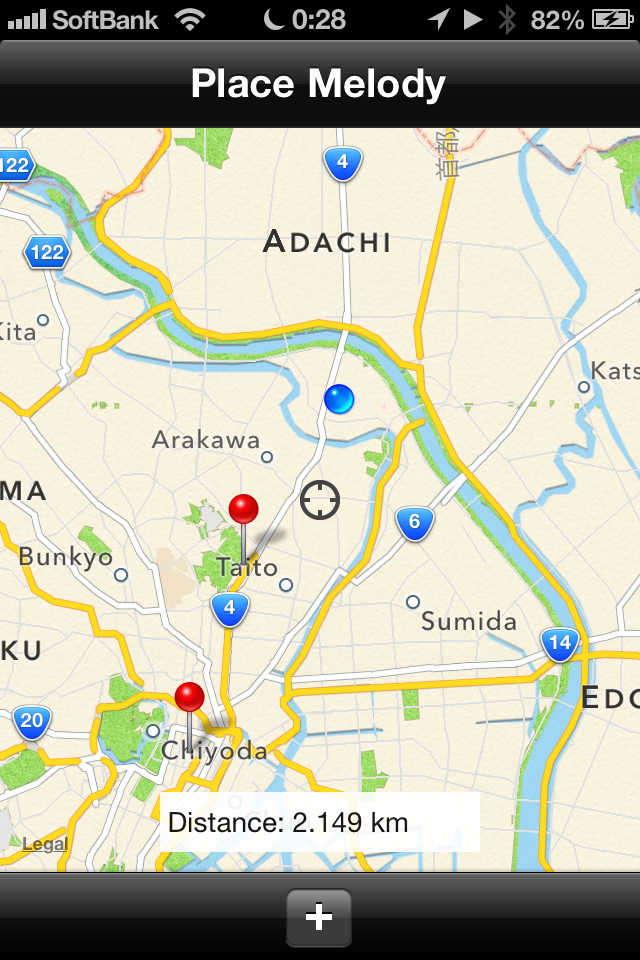
\includegraphics[width=5.866cm]{placeMelody.png}
\caption{Place Melodyのインターフェース}
\label{placeMelody_interface}
\end{center}
\end{figure}


\item
時刻・シーン

音楽の再生時刻とシーンから推薦する方式。
\subsection{OtO}
ユーザーが楽曲を聴いた時間を学習し、図\ref{OtO_playlist}に示すように、
曜日毎に0時から24時までを1時間区切りでプレイリストをつくる。
ユーザーが自動的に再生したいときは、シーンを選択して、
その時刻にそのシーンで以前聴いた音楽のなかからランダムで楽曲が選ばれて再生される。
Mac用のアプリケーションでiTunesと連携している。

\begin{figure}[h]
\begin{center}
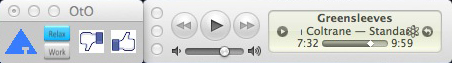
\includegraphics[width=5.866cm]{OtO_imageView.jpg}
\caption{OtOのインターフェース}
\label{OtO_interface}
\end{center}
\end{figure}

\begin{figure}[h]
\begin{center}
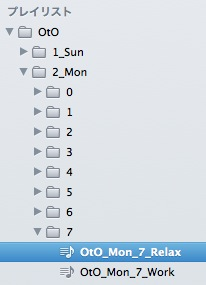
\includegraphics[width=5.866cm]{OtO_playList.jpg}
\caption{OtOのプレイリスト}
\label{OtO_playlist}
\end{center}
\end{figure}


音楽を再生する際にシーンを選択してもらうことによりシーンにあった音楽を推薦する方式。
\end{enumerate}

以上の音楽アプリケーションのプロトタイプを体験してみて、
場所については、場所によって異なる音楽を聴いていることもあったが、
それは、場所自体に直接的な意味合いがあるというよりも、その時刻にその場所にいることが多いという、間接的な関係であり、時刻に比べて相関が薄かった。
例えば、移動中であったときは、状況は移動中であるだけなのにもかかわらず、移動している場所にちりばめられるといったことが起こった。
また、同じ場所であっても、休憩中や、作業中などの様々なシーンに応じて音楽を選んでいる場合でも、一元化されてしまうといった問題点もあった。
シーンを選ぶものは、ユーザー自身で音楽のモードを選んで、選択してもらうことから、実際にはプレイリストを自作する行為に似ており、
リコメンドサービスとしてのメリットが小さくなってしまった。
また、楽曲をシーンに分類するためには、ユーザーが特定のシーンを選択する行為の膨大な学習期間を要することも問題だった。
時刻に関しては、場所、シーンの両方ともに関係しており、
音楽をかける際に、ユーザーの状況を説明するのに、最も基本的な要素であり、直接的だったため、
本研究では時間について特に注目して調べることにした。
このことにより、この研究成果が、場所情報と組み合わせることで状況をより正確に推測したり、
シーンを時間から推測したりといった拡張性に期待したいと考えた。

\subsection{既知の障害}
人によって、生活が不規則な人もいると容易に推測できるために、時間によって、傾向が出ないことも考えられる。
必ずしも。時間と音楽の再生に相関がある人ばかりではないことも留意しつつ、調べる必要がある。
そのため、音楽の再生時刻だけでなく、普段の生活がどのようになっているのかを直接知る必要がある。
また、iTunesの履歴からは、
シャッフル機能を使用して再生されたのか、
ユーザーの操作によって選択されて再生されたのかを、
区別して分析することは難しいので、
再生履歴を一元的にユーザーによる積極的な選択としてみなすことが出来ない場合も注意する必要がある。
また、ソフトの仕様により、履歴情報が全て記録されていない場合があり、
今回使用したiTunesでは、ひとつの楽曲に対して、最後に再生した時刻だけしか記録されていない。
全てを保存するアプリケーションを自作することも可能だったが、
その場合、従来の音楽再生スタイル自体を大きく変化させてしまうことで、
従来の履歴情報を取得することが困難になると考えたため、
この点においては妥協してiTuensを使用することにした。
音楽再生のスタイルがユーザーインターフェースに依存してしまう可能性があるが、
iTunesは音楽を選択する自由度が高いので、iTunes自体が音楽の聴き方を制限することがないと考えた。

また、ジャンル名を取得できていない楽曲もあり、
またユーザーが手動で設定しなくても、iTunesが自動的につけるために、
ユーザーが考える楽曲のジャンルと、iTunesが付けたジャンルとが必ずしも合致するとも限らない。
\subsection{先行研究}
膨大な音楽ライブラリーから今聴きたい音楽を推薦するシステムは、
産総研の後藤真孝さんのMusicreamのように、インターフェースによって音楽を選択する支援をするものや、
楽曲のジャンルの関連性を取得するGeniusなどのサービス、
また、ユーザーが楽曲から受ける印象を集めることで、
音楽の印象から、気分にあった音楽を選ぶことのできるMusicoveryなどのサービスがある。
図\ref{musicovery_interface}に示すのがMusicoveryのインターフェースだが、
4つの方向にそれぞれ、Dark, Energetic, Positive, Calmと、音楽の雰囲気が書かれており、
ユーザーが聴きたい音楽の雰囲気を平面上で選ぶことができる。
このことによって、ユーザーが楽曲を直接選ぶのではなく、雰囲気を決めることで、結果として音楽を選ぶことになるのである。

%musicovery.png
%iPhone W: 58.66mm
\begin{figure}[h]
\begin{center}
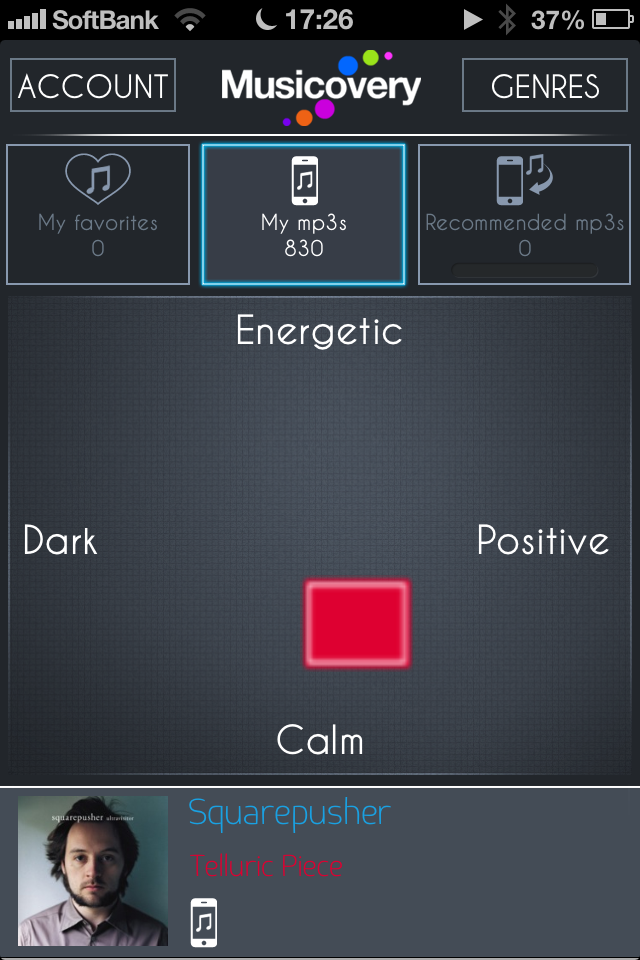
\includegraphics[width=5.866cm]{musicovery.png}
\caption{Musicoveryのインターフェース}
\label{musicovery_interface}
\end{center}
\end{figure}

\subsection{研究動機}
ユーザーの状況を推測することは容易ではない。
また、ユーザーの状況をユーザー自身が入力することも容易ではない。
そのため、ユーザーの状況を推測することが可能であり、ユーザーの入力負担が小さいものが求められる。
いくつかのプロトタイプアプリケーションを試したことから、時間情報が有効であると判断した。
特別なセンサーも不要なためリコメンドサービスにも容易に役立てることができる。
音楽推薦サービスに有用かどうかを調べるために、
時刻と音楽がどのように関係しているのか、関係していないかを明らかにする。

以前は例えば自宅で夜、音楽鑑賞するといった決まった状況で聴いていたため、
音楽を再生する状況に外的な別段の変化はなかった。
しかし、モバイルプレイヤーにおける音楽の再生は、場所や時間を選ばない。
そのため、モバイルプレイヤーの使用者は様々な場所や時間において、自分で音楽を再生する音楽を選択する必要がでてきた。
ユーザーは、状況が変化すると、音楽を再生する同期や気分などに差が大きく出ると思われる。
そこで、外的な状況の変化に対して、音楽の再生がどのように変化しているのかを調べることにした。
\subsection{方針}
本研究では特に時刻に注目して、時刻によって音楽の聴き方がどのように変化するのかを調べた。
時刻に注目した理由は以下の通りである。
\begin{itemize}
\item
規則的、周期的である。
ほとんどの場合、朝は自宅から始まり、夜は再び、自宅にもどる。
その時間も人によってではあるが、パターン化されていると考えられる。
そのため、時刻だけからもある程度、人の営みを推測することができそうだと推測できた。
\item
音楽と相関がありそうである。
現状で、モーニングコンサートや、オールナイトコンサートなど、時刻を表す言葉を冠したものや、
ジャズや、ダンスのクラブは夜行われていることが多く、時刻と音楽のシーンは見慣れている。
そのため音楽には時刻的な要素が存在していると予測できた。
\end{itemize}

\subsection{期待される成果}
この研究が音楽の自動選曲システムの向上に貢献できればと考える。
\subsection{キーワード}
iTunes, iPod, 時間情報, レコメンドサービス, ライフログ

\section{分析手順}
本実験の被験者は普段iTunesを利用して音楽を聴く20代の20名の大学生ある。
被験者は普段から、iTunesと同期しているモバイルプレイヤー(iPod, iPhoneなどのアップル社製の機器)を利用している。

スマートフォンに関しては、インターネット白書2011によると、
所有しているスマートフォンはiPhoneが47.7\%と最も高いこともあり、
多くの人がiTunesをモバイルでも利用していることが推測されることと、
履歴データを調べるにあたって、ラップトップなどを使って、
自宅で音楽を再生した情報と、モバイルで音楽を再生した情報が、
どちらもiTunesで管理されているため、iTunesに限定することにした。

\begin{enumerate}
\item
被験者10名(iTunesをいつも利用して音楽を聴いている大学生)から履歴ファイル(xmlファイル)をメール添付でもらう。

\item
被験者に自分の生活を曜日毎にアンケートシートに書いてもらう。
\begin{figure}[htbp]
\begin{center}
\fbox{							
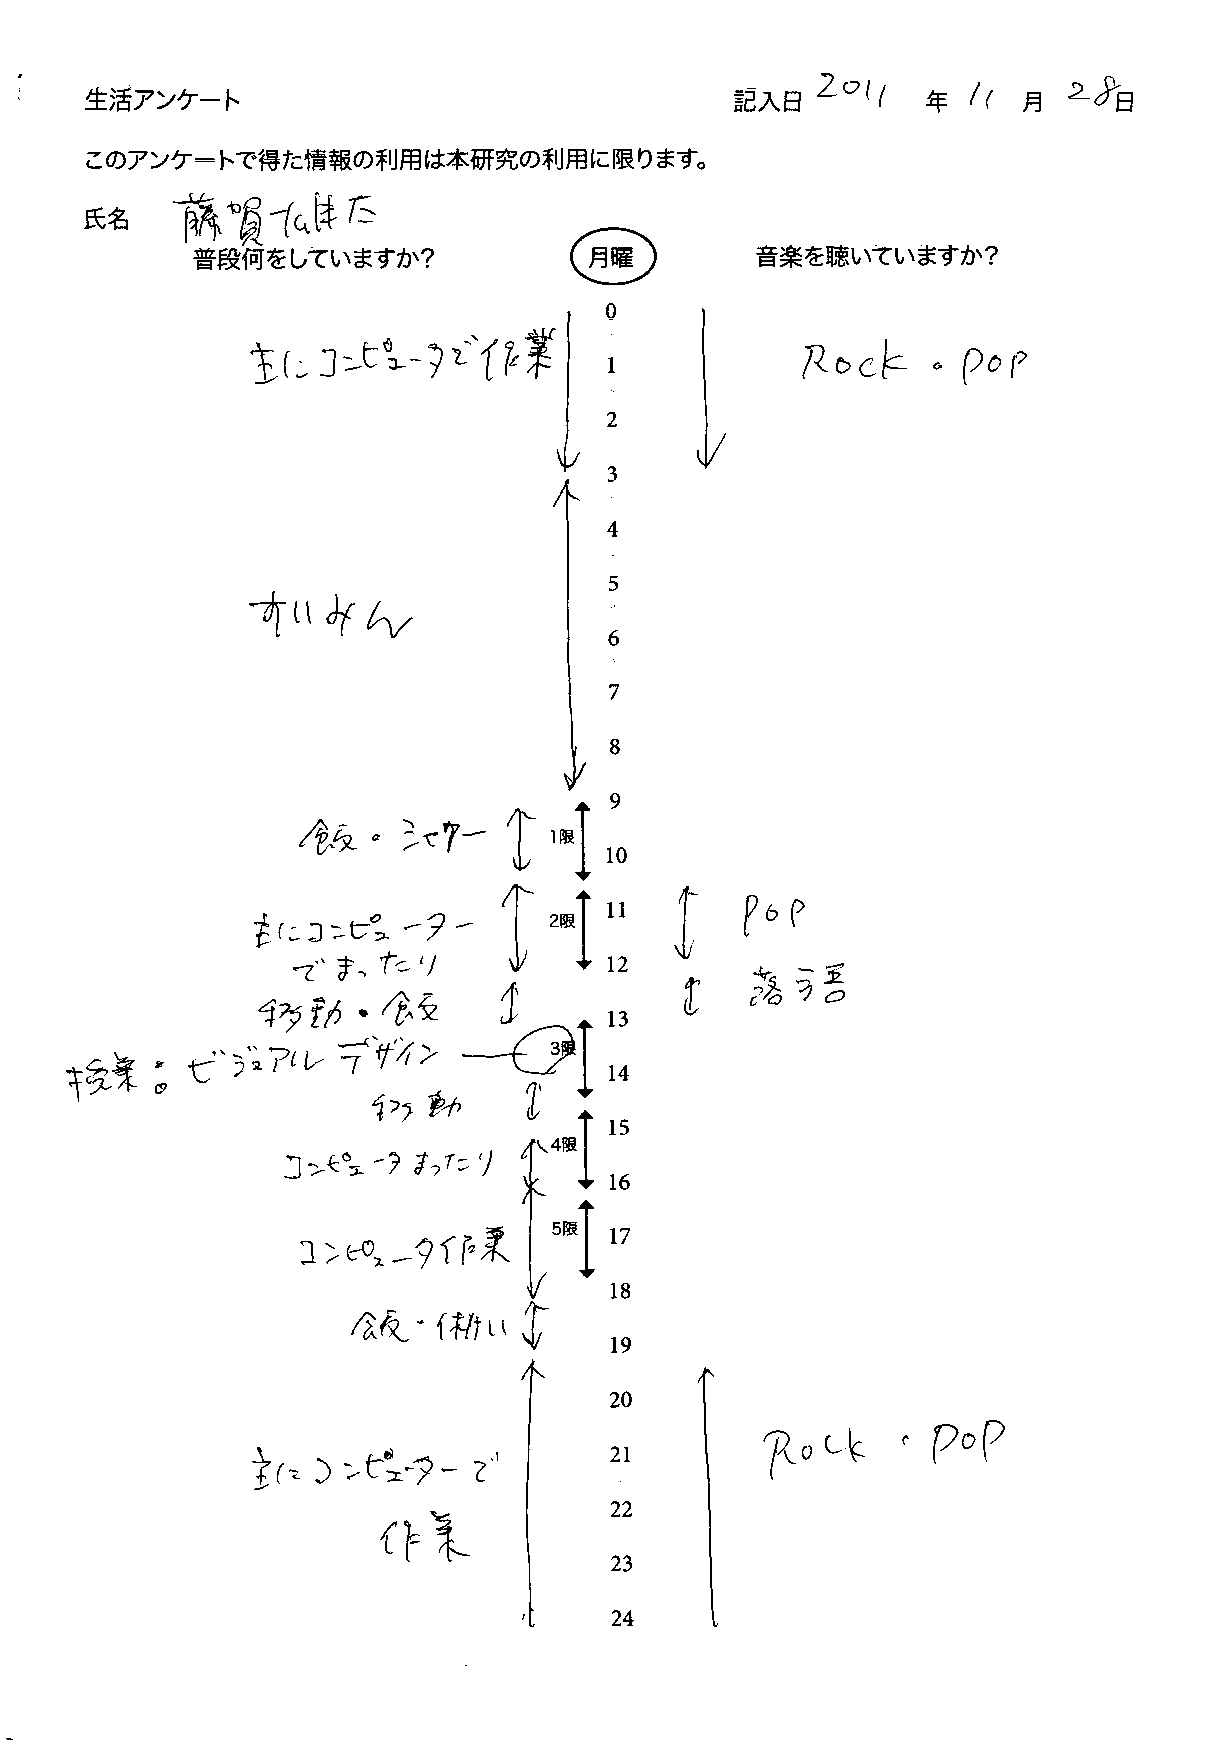
\includegraphics[width=7cm]{musicLifeSheet_sample.pdf}
}
\caption{アンケートシートのサンプル}
\end{center}
\end{figure}

被験者に渡したのは、0時から24時までを30分刻みで目盛りを付けたもので、
普段の生活と、普段の音楽聴取を記入してもらうもので、月曜日から日曜日までの合計7枚のものである。
不規則な生活、気まぐれな音楽再生など、毎週規則正しく定期的に書けない部分も備考として記入してもらう。
なお、iTunesをシャッフルの機能を利用して聴いたかどうかは、iTunesに記録されていないため、備考に書いてもらう。
\item
履歴ファイルから、以下の情報を読み取って、グラフをつくる。
\begin{itemize}
\item
楽曲のジャンル
\item
最後に聴いた日付・時間
%\item
%再生回数
\end{itemize}

\begin{figure}
\begin{center}
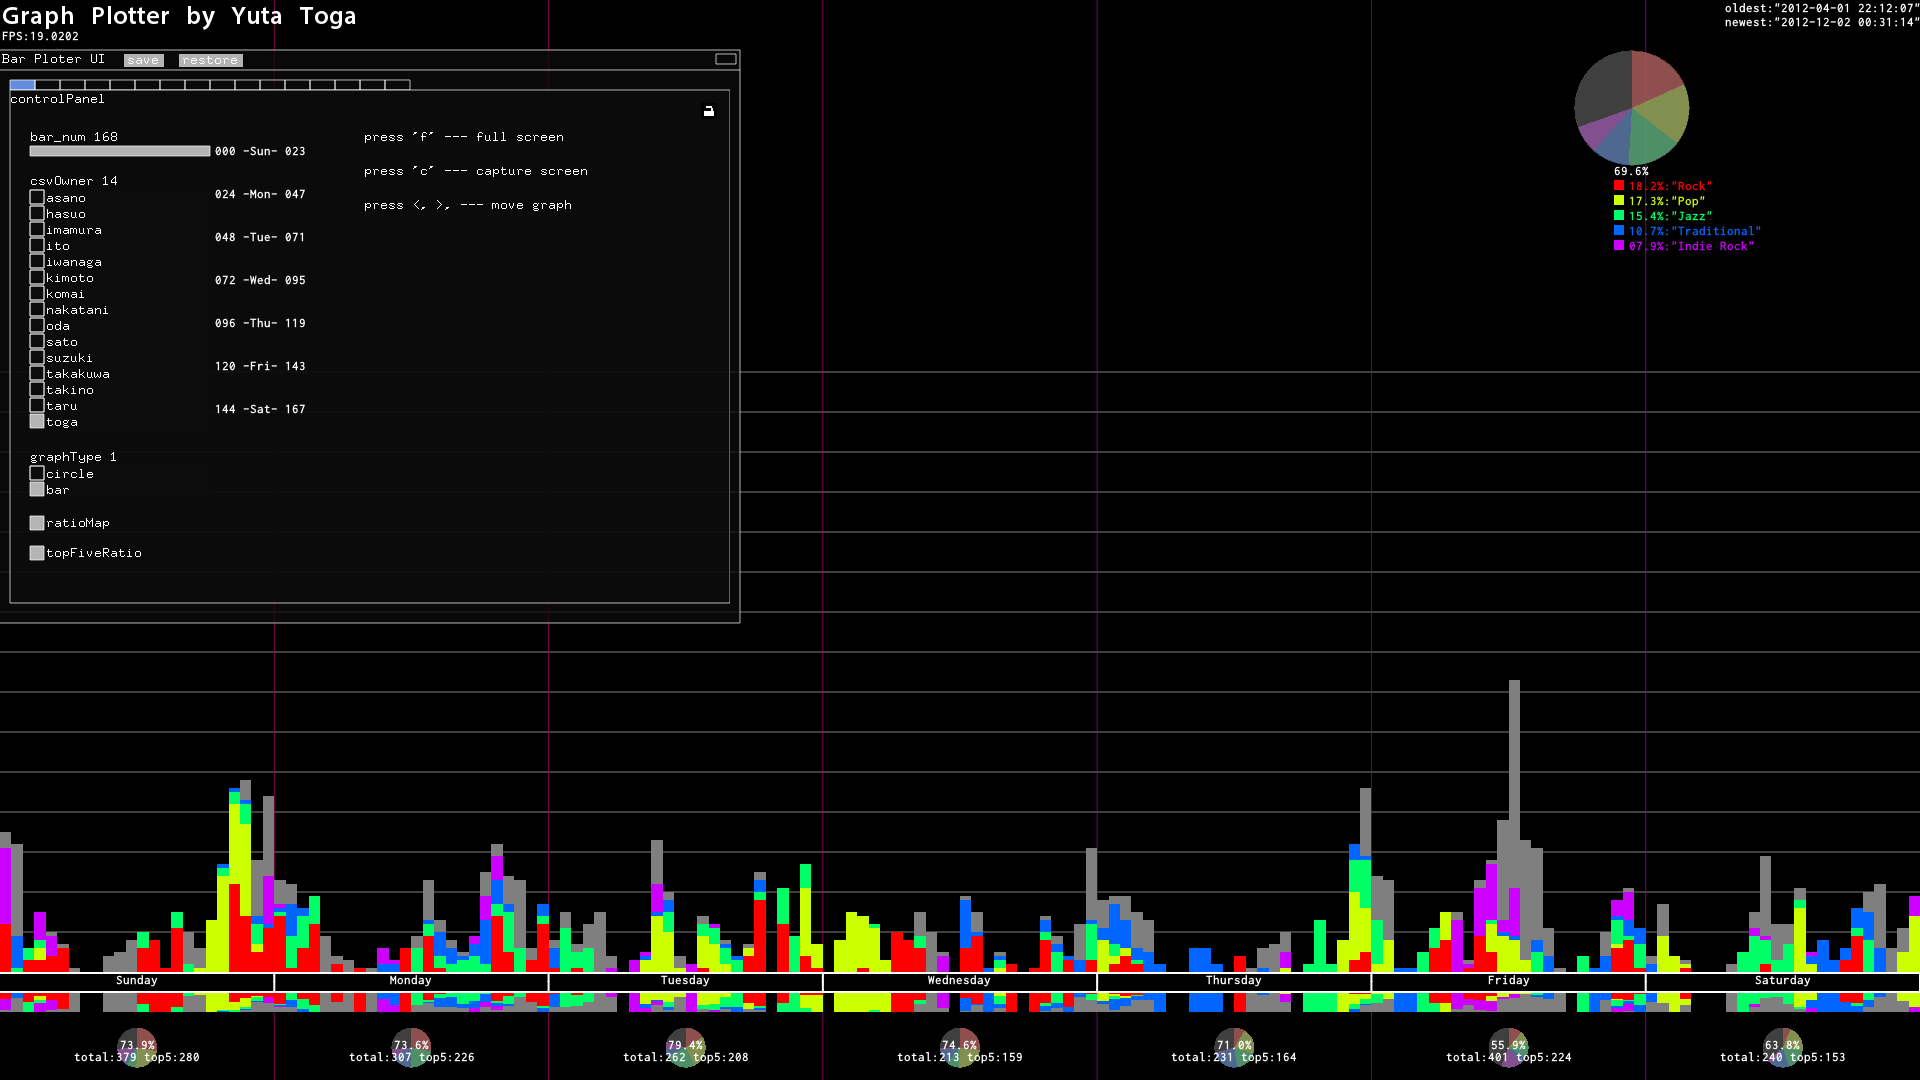
\includegraphics[width=7cm]{graph_sample.png}
\caption{分析結果のグラフの一例}
\end{center}
\end{figure}

\item
被験者のアンケートシートで得た情報と、グラフから読み取ったものとを比較しながら分析を行う。
\item
質問が出た場合は適宜インタビューを行う。

\end{enumerate}


\subsection{曜日について}
本研究の中での曜日は、被験者によって定義が異なる。
通常であれば、1つの曜日の範囲は0時0分から24時0分であるが、
本研究では、音楽を聞いて時間帯を睡眠時間と推測できるほか、
アンケート用紙にて普段の睡眠時間を曜日ごとに教えてもらっているため、
個人毎に起きている時間帯を曜日の範囲として定義した。
そのため、曜日によっては24時間よりも長くなったり、短くなったりしている。
また、0時0分からではなく、
起床したと思われる時間を曜日の開始、24時0分ではなく、
就寝したと思われる時間を曜日の終わりと定義した。
その後、アンケートを見て、
自己申告した情報と、音楽の履歴情報から得られた情報と異なる点、合致する点を比べた。
合致すればするほど、音楽の情報だけで、ユーザーの生活周期を推測できているとみなせるため、
リコメンドサービスに有効であると考えられる。

\subsection{音楽について}
本研究の中では、音楽または楽曲という定義を、iTunesの中でのミュージックを流用する。
そのため、楽曲以外にも、落語や、ラジオドラマ(オーディオドラマ)、英会話の音声を含む。

\subsection{グラフと、アンケートシートの比較}
グラフからは音楽を聴くという容疑毎の時刻幅を推測できる。
特に推測が難しいところは、深夜なのか早朝なのかわからない時間帯に音楽が聴かれている場合である。
そこで、アンケートシートを参考にしてどちらなのかを決定する。
また、生活が不規則または、音楽を可けっぱなしにして聴くという人は、
どこに切れ目があるのかを決定できないということもあった。
アンケートシートには、音楽を聴いている時刻幅と、生活項目が書かれた時刻幅がそれぞれ書かれてあるため、
グラフによる音楽試聴の時刻幅と3種類の時刻幅ができる、それぞれを比較して、
実際の音楽視聴
ユーザーが自供する音楽試聴
生活との関係性。
実際の生活との関係性。
	実は本当の生活リズム自体が書かれているかどうかも怪しいという点を注意しなくてはいけない。
	
	
どこまでノイズを取り除いていいのか問題。



\section{結果}

寝ている間に聴く、または、生活が極端に不規則という人以外の多数は寝ている時間がおおよそ推測できる。
必ず聴いていない時間が存在することがあり、その時間はバイトや授業などが毎週あることが多かった。
また、毎週決まって聴く時間があると、その場所だけ、再生回数が群を抜いて大きくなる。
そのため、数回しか聴いてない情報を省いて分析をすると、
定期的に音楽を聴く時間帯が見えてくる。

また、人によっては金曜の夜だけ多く聴いているというような、曜日による偏りが見られた。
個人単位で大きくことまる音楽の聴き方をしており、被験者の数もパターン化するほど多くなかったため、
具体的に特徴的な人の例を以下に示すことにする。
\subsection{規則的な人}
規則的な人は、図\ref{sample_regular}のグラフに示すように時間に決まった時間に音楽を聴いている。
規則的に音楽を聴く人は、アンケートシートで調べた普段の生活も、非常に規則正しい生活をしている。
特に、寝る時間や、起きる時間、外出する時間、帰宅する時間が規則正しいので、
聴いていない時間はほとんどきいておらず、聴いている時間はかなり聴いているため、凹凸の激しいグラフとなっているのがわかる。
寝ている時間が音楽を聴いていない時間帯から容易に推測することができる。

\begin{figure}[h]
\begin{center}
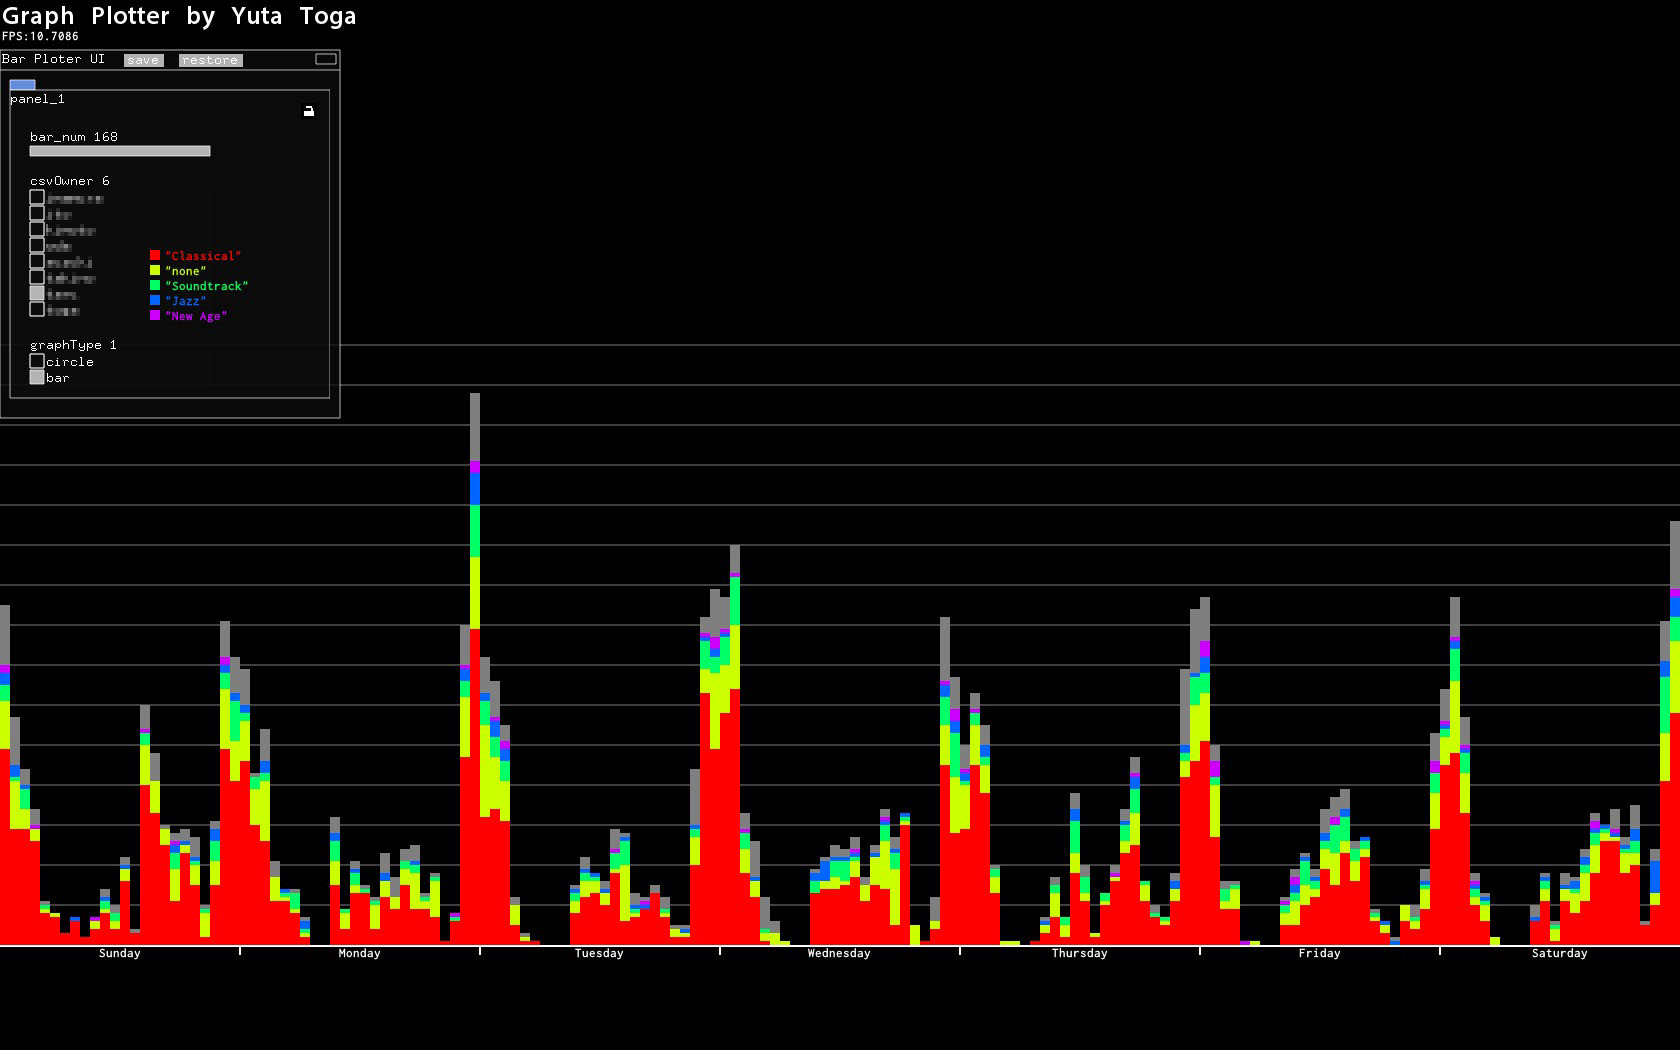
\includegraphics[width=7cm]{sample_regular.jpg}
\caption{規則的な人の例}
\label{sample_regular}
\end{center}
\end{figure}



\subsection{不規則な人}
不規則な人は、図\ref{sample_irregular}のグラフに示すように時間によって音楽の試聴のリズムは見られない。
深夜アルバイトをしている学生が、翌日数時間を複数回に分けて睡眠するといったことも見られ、曜日をその人における7つの曜日を設定することが難しい例もあった。
曜日によって、ばらばらになっている。
音楽によって、睡眠時間を推測することが困難で、どこに曜日の切れ目があるのかすら曖昧である。
こういったユーザーには再生を自動的にオンオフするような推薦機能はおすすめできない。

\begin{figure}[h]
\begin{center}
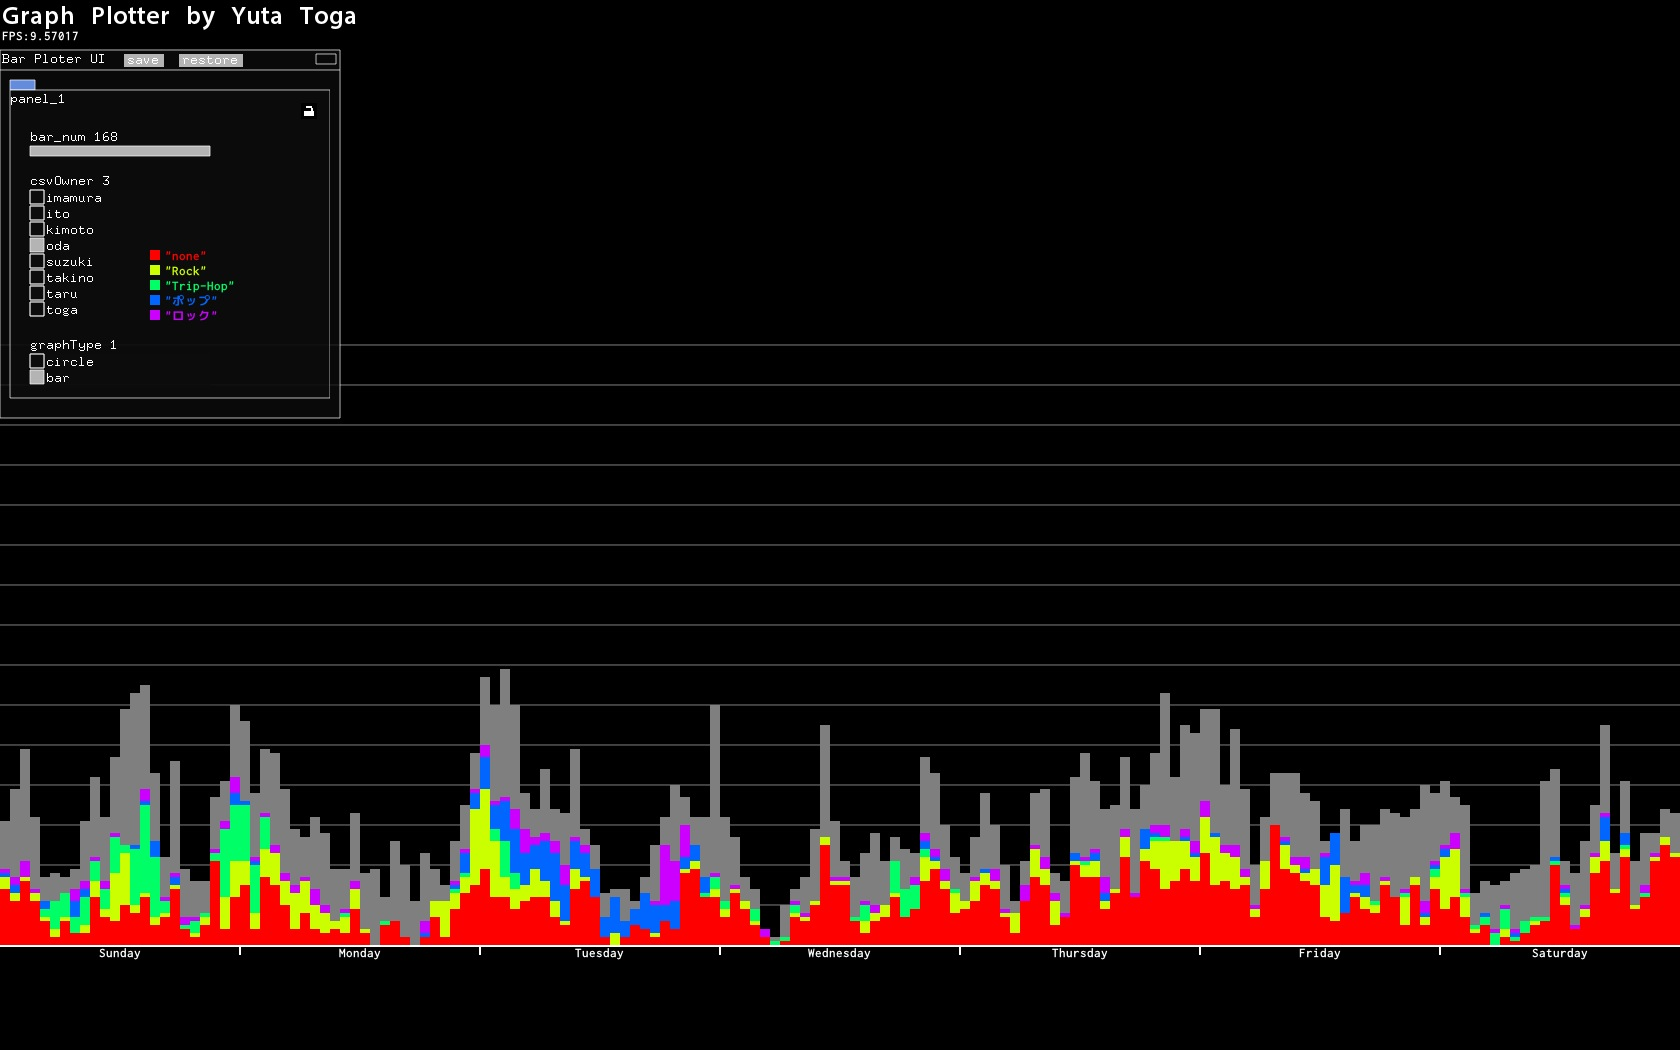
\includegraphics[width=7cm]{sample_irregular.jpg}
\caption{不規則な人の例}
\label{sample_irregular}
\end{center}
\end{figure}

\subsection{音楽ジャンルの分布が一定な人}
図\ref{genreMap_regular}のグラフに示すように、高さを見なかった場合、一定なパターンもある。
それは、この場合、シャッフル機能を利用して再生しているために、
iTunesに入っている音楽ライブラリのジャンル構成がそのまま音楽の再生の分布になっていると考えられる。
こういった分布を取る人に対しては、何を選ぶを支援するのではなく、どのタイミングで再生すべきか、停止すべきかを支援するのがよいと思われる。
音楽の停止と再生の切り替えだけでは、ユーザーが受ける便利さは小さいように思えるが、
タイマーのように音楽の開始によって、行動を促したり、時間を示したりといったインタラクションが起きることが良い点である。

\begin{figure}[h]
\begin{center}
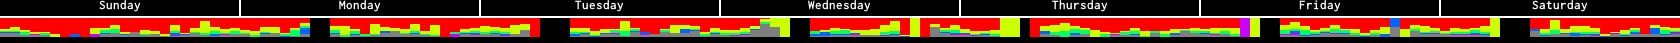
\includegraphics[width=7cm]{genreMap_regular.jpg}
\caption{音楽ジャンルの分布が一定な人の例}
\label{genreMap_regular}
\end{center}
\end{figure}

\subsection{音楽ジャンルの分布むらがある人}
\begin{figure}[h]
\begin{center}
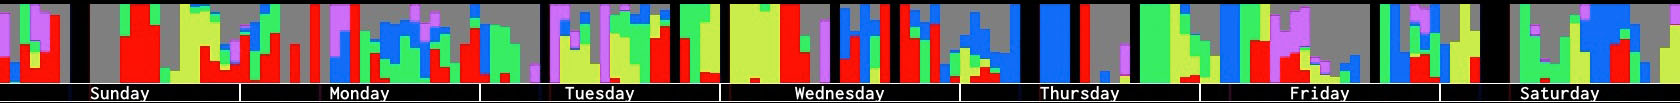
\includegraphics[width=7cm]{genreMap_irregular.jpg}
\caption{音楽ジャンルの分布にむらがある人の例}
\label{genreMap_irregular}
\end{center}
\end{figure}

\subsection{ジャンル派(偏食型)}


\begin{figure}[h]
\begin{center}
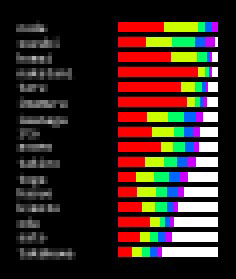
\includegraphics[width=7cm]{sortedOther.jpg}
\caption{iTunesのなかのライブラリーのジャンルの内訳全員分}
\label{sortedOther}
\end{center}
\end{figure}


ジャンルトップファイブが占める比率を出した結果、ジャンルの上位が多くを占めている場合がある。
特に、ベスト1、ベスト2によって、ほとんどを占める人に対しては、
曜日や時間によって偏りがある場合は、ジャンルによる音楽リコメンドだけで十分だと考えられ、
曜日や時刻によって偏りがない場合は、シャッフル機能による再生で十分だと考えられる。
\begin{figure}[h]
\begin{center}
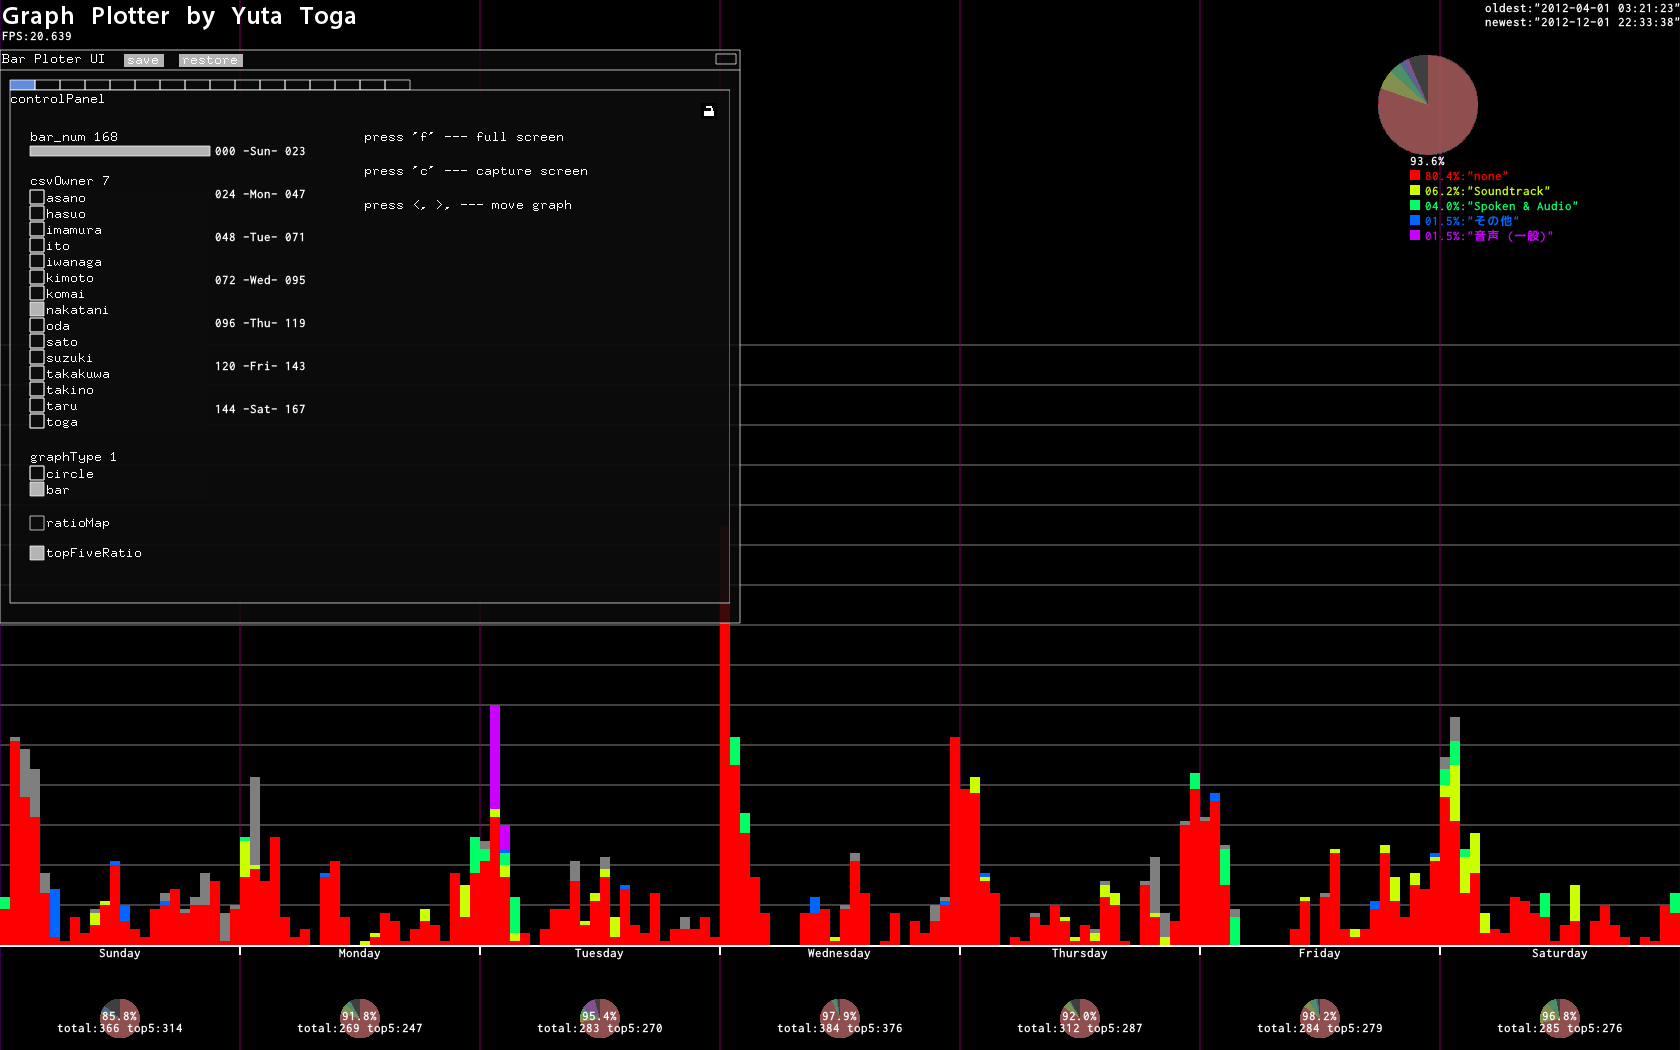
\includegraphics[width=7cm]{topFive_heavy.png}
\caption{上位のジャンルによって多くを占めている人グラフの例}
\label{topFive_heavy}
\end{center}
\end{figure}

\subsection{ノンジャンル派(雑色型)}
ジャンルの上位が占める比率を出した結果、
ジャンルの上位が占める割合が小さい場合。
この場合、ジャンルから選んだり、推薦することによる効果が小さいので、ジャンル以外の要素を使ったリコメンドが有効だと考えられる。
ジャンルによって音楽を聴いていないと考えることもできる。
iTuensにおいてチェックマークの入っている音楽全体のジャンルの内訳と、曜日毎のジャンルの内訳を比べると違いが大きい。
このため、このユーザーはシャッフル機能による再生をするのではなく、自分で積極的に選択しているものと考えられる。
こういったユーザーへは、曜日と時刻から推測される楽曲を推薦することで、
普段聴いているような音楽を再生することができると考えられる。

\begin{figure}[h]
\begin{center}
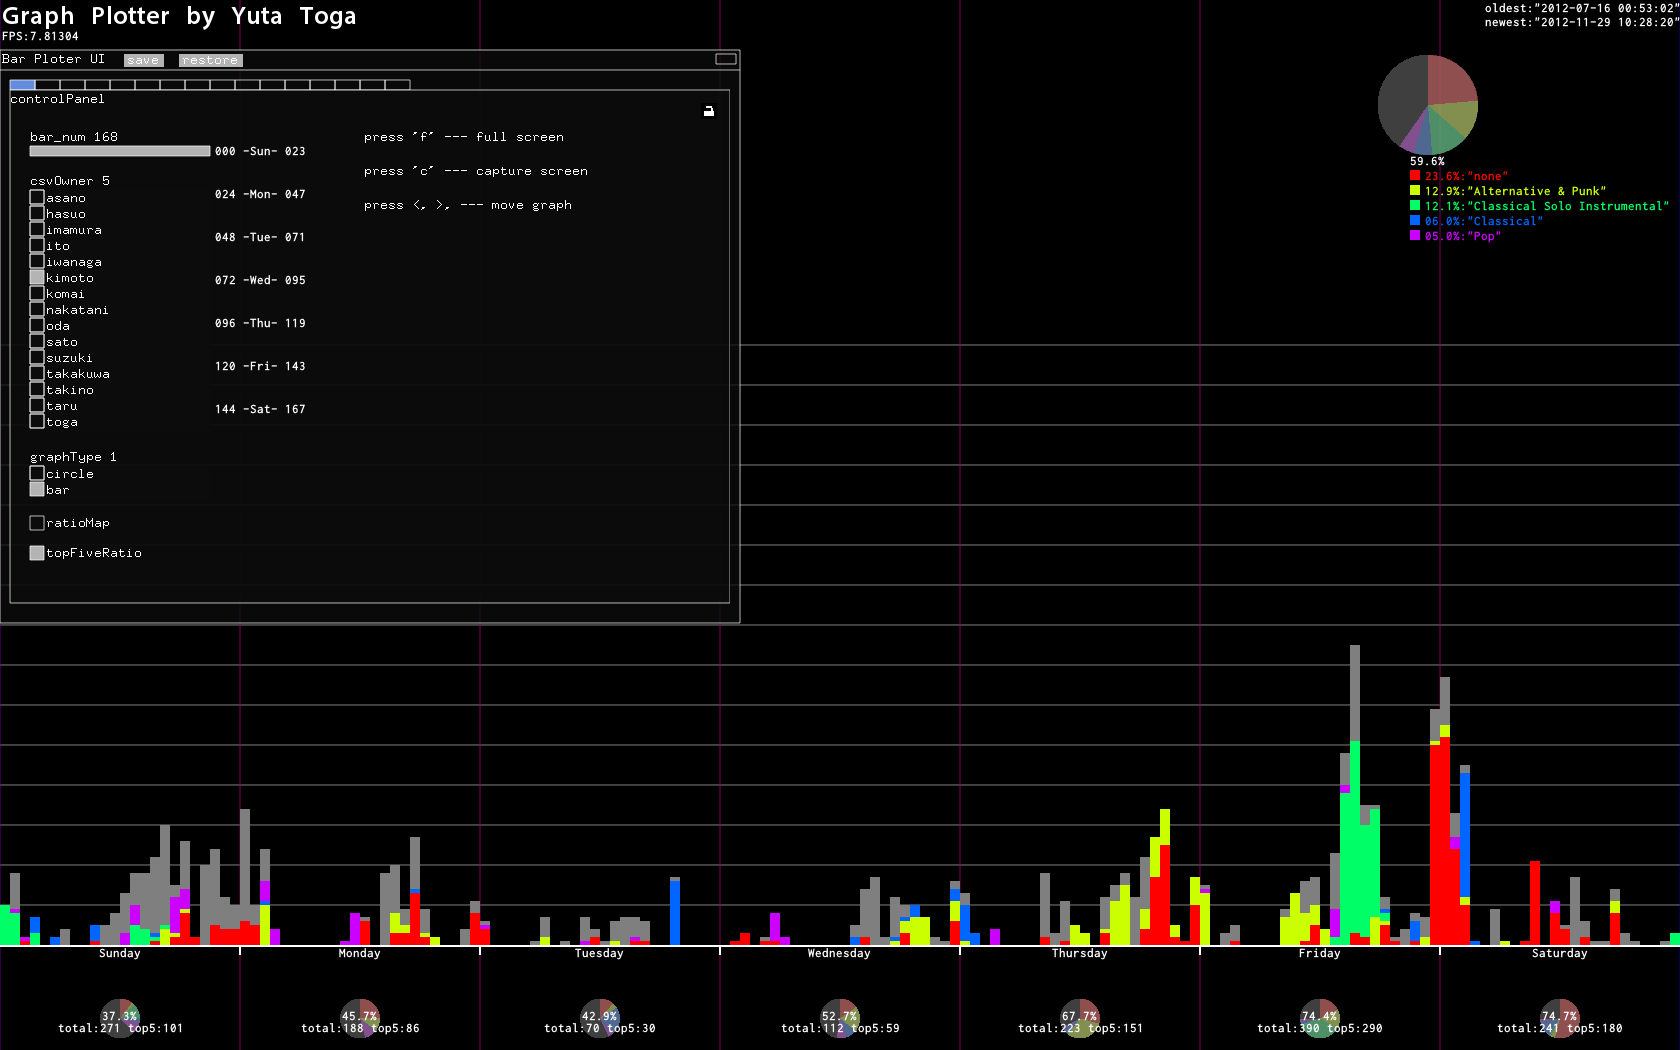
\includegraphics[width=7cm]{topFive_light.png}
\caption{上位のジャンルによって占められる割合が小さい人グラフの例}
\label{topFive_heavy}
\end{center}
\end{figure}

\subsection{音楽をあまり聴かない人}
図\ref{lightListner}に示すようにあまり聞かない人は、曜日ごとのトップ5が占める比率も80%を超えることが多い。

\begin{figure}[h]
\begin{center}
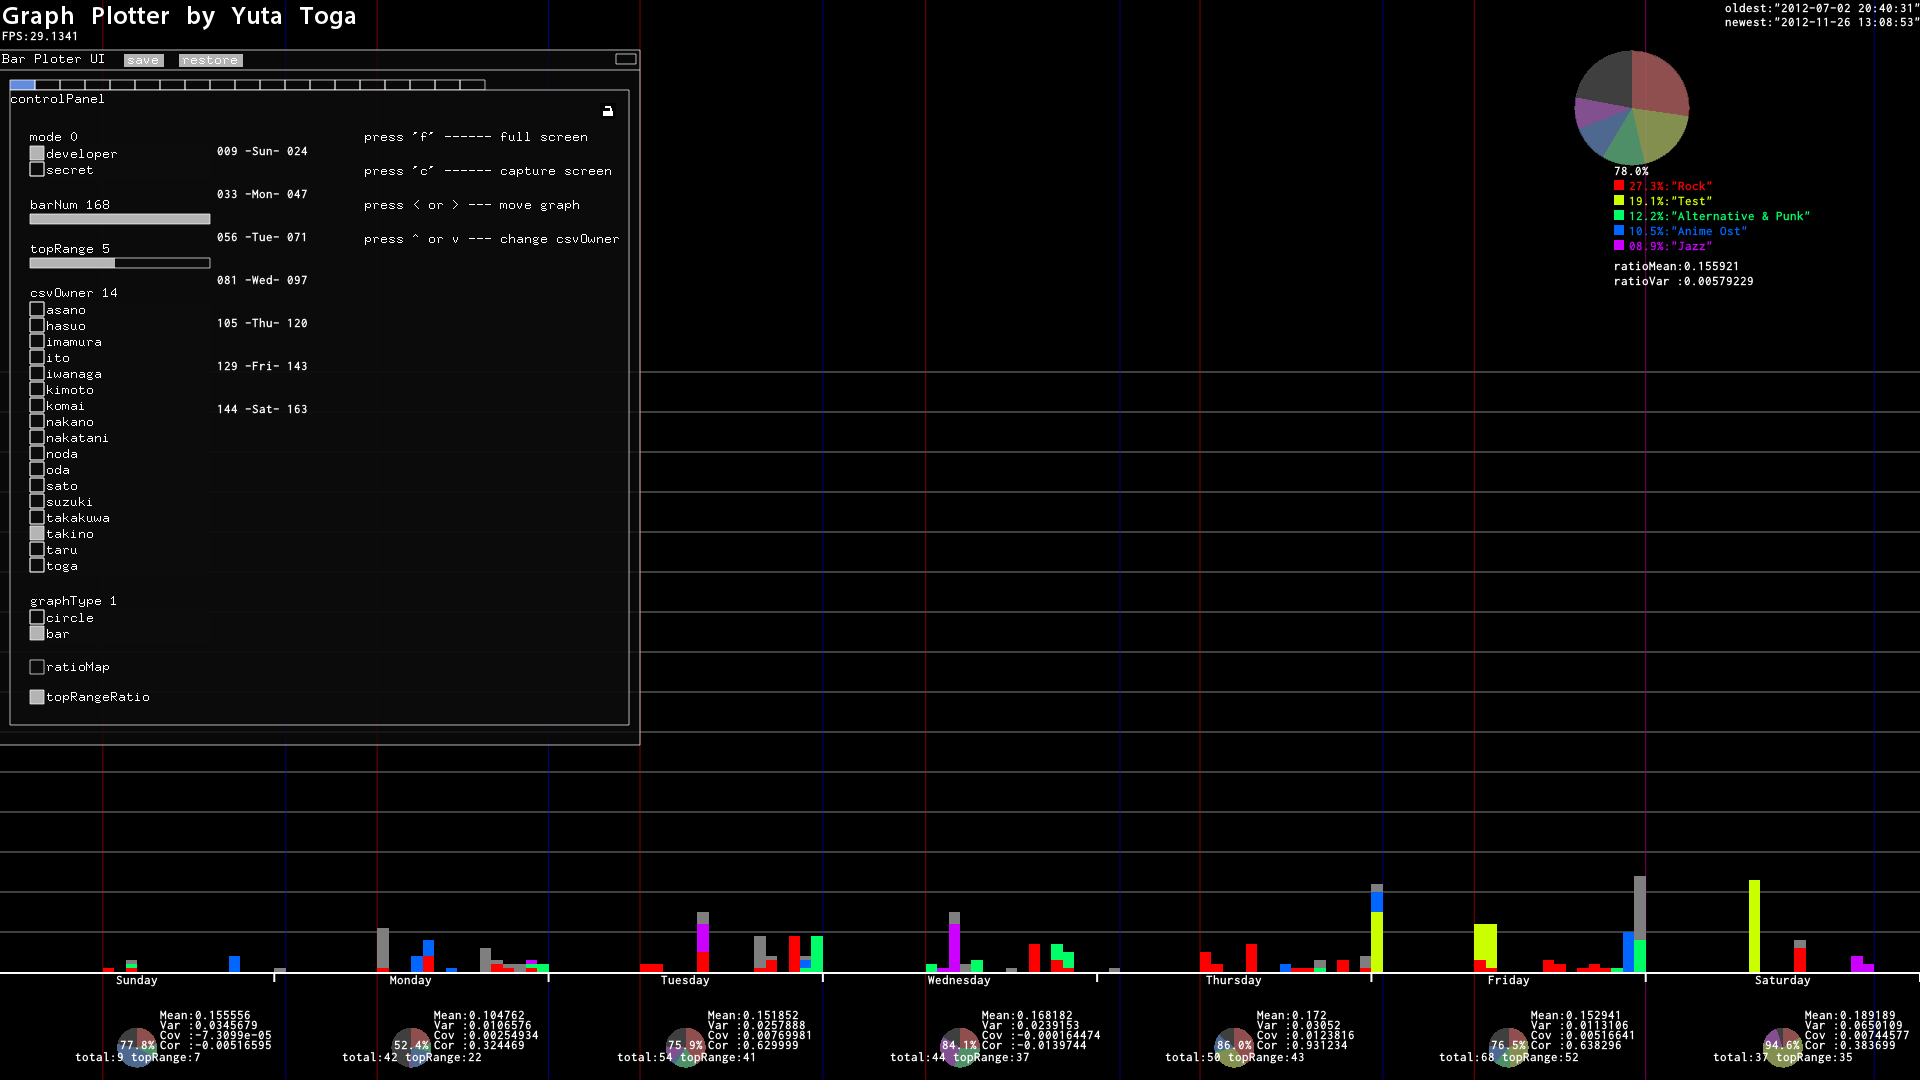
\includegraphics[width=7cm]{takino.png}
\caption{上位のジャンルによって占められる割合が小さい人グラフの例}
\label{lightListner}
\end{center}
\end{figure}


\subsection{シャッフル機能を使う人のチェックマークの入った楽曲の例}
図\ref{checkedItemsGenreMap_shuffle}と図\ref{weekGenreMap_shuffle}を見比べると、
曜日毎に再生されたジャンルの内訳がiTunes内のチェックマークの入っている楽曲全てのジャンルの内訳、
すなわちランダム再生で再々されるジャンル毎の再生確率とほとんど同じになっているのがわかる。
このため、このユーザーは音楽をシャッフル機能を使用して再生しているのがわかる。

\begin{figure}[h]
\begin{center}
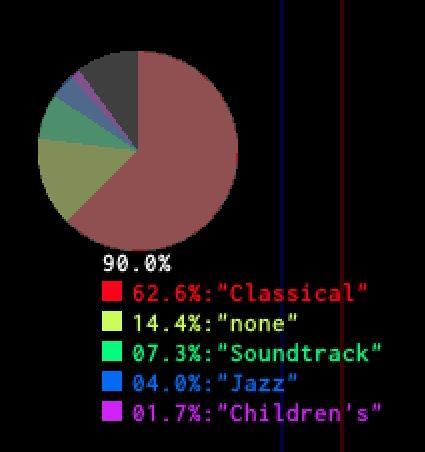
\includegraphics[width=7cm]{taru_checkedItemGenreRatio.jpg}
\caption{シャッフル機能を使う人のチェックマークの入った楽曲の例}
\label{checkedItemsGenreMap_shuffle}
\end{center}
\end{figure}

\begin{figure}[h]
\begin{center}
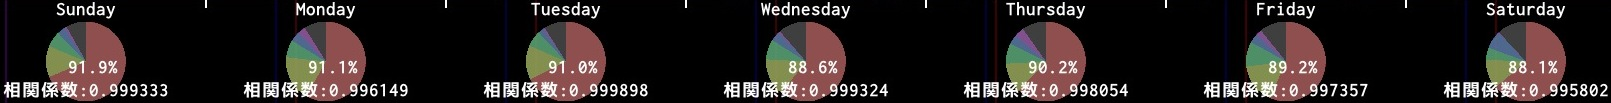
\includegraphics[width=7cm]{taru_weekGenreRatio.jpg}
\caption{シャッフル機能を使う人の曜日毎のジャンル内訳の例}
\label{weekGenreMap_shuffle}
\end{center}
\end{figure}

\section{分析}
iTunesの仕様により、再生履歴は最後に聞いた時間の情報しか残っていない。
例えば、10回聞いたの楽曲がある場合も、
いつ聞いたのかという情報は最後の10回目しか記録されておらず、
1回目から9回目の情報は上書きによって失われている。
そのため、今回の研究では、アンケートにおいて、シャッフル機能を使用しているかどうかを聞き出すことにした。
もし、月曜日に特に音楽を聞いているという場合、
なぜ月曜にそうなるのかという理由は聴いてみないとわからないため、アンケートによって得られた普段の生活を参照した。
また、この時間あなたはなんらかの理由で音楽を聴けない状況ではないですか?
というように音楽試聴における状況について、予想される状況をインタビューすることによって、被験者がアンケートで自供した情報より多くのことを得ることができた。
これは、今後、自動選曲システムにおいて、設定をすべてユーザーに任せるのではなく、
もしかして、金曜の夜はあまりロックは聴かないですね?というような、質問形式で数問回答させることにより、
ユーザーの音楽試聴状況に沿った選曲ができる(沿うことがよいリコメンドかどうかは別として)可能性を示唆する。
これは、自覚して供述可能なこと以上のことを推薦システムを利用することで、引き出すことができる可能性があるということである。

ここでは、ランダムに再生している人と、時間と音楽再生に偏り(相関がある)人にどう分かれるのかを調べる。
\subsection{曜日毎に再生されたものと、音楽ライブラリのジャンルの相関}

図\ref{corTable}は、曜日毎に再生されたジャンルの内訳と、音楽ライブラリ全体のジャンルの内訳の相関を示したものである。
右の表の数は相関係数を示している。横軸が曜日、縦軸はユーザを示している。
左に見える棒グラフは、ユーザの使っている音楽ライブラリ全体の音楽、すなわち、シャッフル機能で再生される可能性がある楽曲のジャンルの内訳を示している。
色は、1つのジャンルを表しており、
赤色は1番目、黄色は2番目、緑色は3番目、青色は4番目、紫色は5番目に多いジャンルを表しており、
白はその他のジャンルをまとめている。
右の表は0.8以上の値の場合、赤いハイライトを施してある。
これを見ると、曜日に関係なく、
音楽ライブラリ全体と相関が高い音楽再生を行う人が、
ユーザーが持っているジャンルの内訳に関わらず、
存在することがわかる。
また、相関が小さいひとは、曜日に関わらず相関が低いことも分かる。
シャッフル機能を利用する人は、必ず相関が高くなっている。
一方、シャッフル機能を使わない人も、相関が高くなる場合が頻出するため、
相関だけで、シャッフル機能をしているかどうかを判断することはできないが、
相関が低いところはユーザーが意図して選んでいることがわかった。
以上のことから、音楽ライブラリー全体と相関が低い曜日がある場合は、
ジャンルによる推薦ではなく、時刻情報に基づく推薦が適切だと考えられる。

シャッフル機能を使わない人であっても、ある曜日に再生された音楽のジャンルの内訳が、音楽ライブラリ全体の内訳と相関が高いケースがある。
これは、音楽ライブラリ自体が、ユーザーの再生したいものだけを追加するものであることから、
再生したい音楽のジャンルの内訳が、意図しなくとも一致してしまった結果であると推測できる。


アンケートシートによると
シャッフル機能は、移動中や作業中など、ながら聴きをしている状況において特に使用されていた。
これは、作業に支障がでてしまうことになるので、音楽再生のための操作をできない、したくないからであると推測できる。


\begin{figure}
\begin{center}
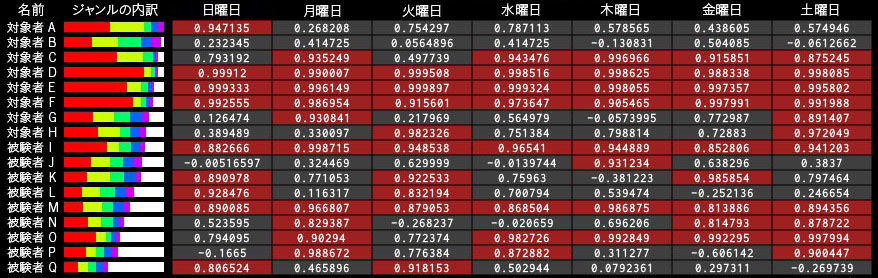
\includegraphics[width = 7cm]{corTable.jpg}
\caption{曜日毎に再生されたものと、音楽ライブラリのジャンルの相関一覧}
\label{corTable}
\end{center}
\end{figure}


\section{考察}


アンケートに書かれている普段の音楽の再生状況と、
iTunesの履歴情報から分析された音楽再生の状況が異なる場合、
一致する場合それぞれについて、なぜそうなるのかを考察する。
生活のコンテキスト、特に時間情報が音楽再生に影響力をもっているかどうかを考察し、
音楽リコメンドサービスについての発展を考える。


寝ている間は聞いていない、授業に出ているときは聞いていないといった、
特定の状況によって、音楽の再生が必ずされていない時間を持っている場合、
音楽の再生履歴だけで、そのひとの生活を推測することが出来る。

聴いていない時間がない場合は、
生活が不規則であるか、
寝ている時間を含めて、音楽を流しっぱなしにしている、
前者は、ユーザーが持つ生活リズムが不定なので、時刻による推薦が困難である。
後者は、時刻によって再生されている音楽のジャンル内訳が、音楽ライブラリと同じジャンルの内訳と同じ場合は
シャッフル機能を使用している可能性が高い。


また、音楽の聴き方は人によってばらつきがあり、
特に、シャッフル機能を使っているかどうかによって、
その差が大きく異なる。

また、そもそもリコメンドサービスをするほどの情報を集められない人もおり、
個人の情報による、個人のためのリコメンドサービスのためには少なくとも、
多量に聴いている人という条件が必要であり、
時刻による楽曲推薦システムは音楽を聴いている時間が長ければ長いほど効果が上がる。

音楽の余り聞かない人に音楽をリコメンドするためには、
そのユーザーに音楽の好みを質問形式で聞いたり、
音楽の聞く頻度や時間帯を質問するなどの問答を繰り返すことにより、
リコメンドすべき時間やジャンルを推測する。

その他の方法は、多くの人の音楽の聴き方を集めて、その人がどんな音楽再生のパターンをもっているのかを調べるのが良い。しかし、そのためには、その人が自分の音楽の聴き方を自分で把握している必要がある。

今回の実験では、本人が自覚していないのにもかかわらず、定期的な音楽の聴き方をしている例も見られているため、
自分で自分が聞きたいものを、一気にそれぞれの時刻についてすべて回答することは容易ではない。
そのため、まずは従来の音楽の聴き方をして、その履歴から、次第にユーザーの好みを学習していくことが望ましい。

本研究ではiTunesを使用したが、
第二章で述べたように履歴情報といっても欠落している情報が多く、
ユーザーがスキップしたかどうかや、
シャッフル機能を使用して再生したのかどうかや、
複数回再生された楽曲の複数回分の再生時刻履歴など
を把握することができなかった。
例えば、スキップしたとすると、
ユーザーはその楽曲を積極的に聴きたくないという意志を表しているため、
ユーザーの好みの学習には直接的に有効である。
そのため、音楽再生プレイヤー自体がユーザーの好みを学習できるように実装されているべきである。
そのためには、ユーザーが自分の操作を保存されることや、
第三者に自分の履歴情報を提供することなどプライバシーなどの問題もあるかもしれないが、
煩雑な操作からの開放、聞きたかった音楽との出会いの推進のために進めていくことが望まれる。

ユーザーが他の活動に支障が出ないようにするためにシャッフル再生をしている場合、
音楽推薦システムを利用するのに適したタイミングであるにもかかわらず、
シャッフル再生を使われることで、
ユーザーの聴きたい情報を取得できないという問題もある。

現在にいたっても単純なシャッフル機能の人気を知ることになったが、
リコメンドとはシャッフル機能以上の効果をもつ何かを持つ必要があるため、
ユーザーの聞きたいものだけを推薦するだけでは単調になってしまうなどのことも考えられる。

というのも、音楽の再生に偏りがあるひとも少なからず他の楽曲も聴いているからである、
そのため、すべてをランダムにするわけでもないが、
好みのジャンルを時間から推測し、ジャンルによって再生確率が動的に変化して、
偏りのあるシャッフル機能にすることを提案したい。
音楽の聴き方は、
アプリケーションのインターフェースによって使い方に偏り
(アクセスしやすい使い方がアプリケーションによって決まってくるということ)
ができることから、時間軸を表示すると時刻の情報から音楽へのアクセスがしやすい場合分析結果が異なってくる可能性はある。
現在はジャンルによるリコメンドが主流であり、
iTunesの音楽の聴き方自体もジャンルから選べるようになっていたりといったふうに、
結果として履歴データもジャンルによってしか情報が現れていない可能性もある。
音楽の聴きたいという思いが、ジャンルへと濃縮され、履歴データを活用してジャンルによる推薦という還元をとることを行うだけでは、ユーザーの音楽再生のコンテキストの一部分でしかないジャンルだけに役割が集中するあまり、
不鮮明な情報に基づく推薦となってしまう。
また、ユーザーの実感が不在な第三者によるジャンル分けは、ユーザーによる可読性も乏しい。
そのため、意味が単純で理解もしやすい時刻という、
身体性のある情報によるリコメンドはユーザーによる訂正やカスタマイズが容易である。
というのも、リコメンドはブラックボックスである必要はなく、
可読性のあるものであれば、ユーザーの対話(質問形式による学習)や。
可読性のあるユーザーの生活周期、
並びに音楽周期をユーザー自身によってリコメンドのアルゴリズム自体を直接調教することができる。
それによって、最終的には、今回の実験の際に記入してもらったアンケートシートのようなものを、
リコメンドを行うアルゴリズムによってつくりながら、
コンピューターがユーザーの状況に合わせて、ユーザーを楽しませることができることを目指したい。

また、注意したいことは、
音楽を毎回積極的に選択しているユーザーは、その分リコメンドサービスによって、選択の支援をすることもできるが、
一方、ユーザーが、選択するという行為それ自体を楽しんでいる場合や、
選択することによって音楽を楽しんでいるとも考えられるため、かえって不必要になる可能性もある。
よって、推薦システムを利用するかどうかは最終的にはユーザー自身が管理できる自由度を持たせるべきである。

\subsection{アンケートシートとの合致}
シャッフル機能を使用してしか聴かないというユーザーのジャンルの内訳は、
その通りにiTunesのジャンルの内訳が、
そのまま音楽再生のジャンルの内訳になっていた。

また、普段の生活の項目の中では、移動や、アルバイトなど、自分以外との活動である場合には、
アンケートで書かれたことと、音楽の履歴情報が合致していることが多かった。
これは、睡眠時間が不規則な人であっても、やらなければいけない仕事などの時間には、規則正しくなるといことで、
個人の中でも不規則的な生活をする時間と、規則的な生活をする時間があるということである。
また、普段の生活の項目の中で、作業中に音楽を聴くと回答した項目は、自分だけの活動でありながら、
アンケートで書かれたことと、音楽の履歴情報が合致していることが多かった。
作業中に関しては、作業用BGMとして音楽をかけて作業するといった、
音楽と作業がセットにすることが習慣化しているからだと考えられる。


\subsection{アンケートシートとの違い}
音楽再生のむらは、
ユーザーが自分で自分が何をどんな時間で聴いているかを知らない。例えば・・・・

\subparagraph{結論}
聴き方は個人で大きく異なっているが、
個人の中では、その人独自の聴き方があることがわかった。
%シャッフル機能について
シャッフル機能を使用した再生が人気なのは、ユーザーの状況や、好みによって、その効果が変化しない点にある。
しかし、それは最大公約数的な良さであって、最適なものだとはいえない。
シャッフル機能よりも、曜日ごとに分けて推薦する方が、
ユーザーのいつもの音楽再生に沿ったものを自動的に再生できる人もいる。
人によって、適切な推薦システムは異なっている。
そして、曜日によってシャッフル機能を使用していたり、選んでいたりするデータもあったことから、
その適切な推薦システムは曜日によっても動的に変化すべきである。
%ジャンルについて
また、聴いているジャンルは、曜日によってむらを持つ人もいるため、
曜日によって動的に変化すべき人もいる。

また、アンケートシートを見なくても、
音楽履歴データのグラフを見ることで、
生活が規則的なのか不規則なのかを推測することができた。
このことは、
朝の音楽や、寝る前の音楽など、音楽を再生するか、停止するかといった、
音楽の選曲ではなく、オンオフという操作の支援において、
有効である人と、無効である人の区別がつくということである。
そのため、履歴データを参照することで、
その人に音楽の操作の推薦をすべきかどうかを推測できる。

\subsection{今後の展望}
普段自分が選んでいるような音楽を、
自動的に再生することが、音楽推薦の最終形であるとは限らない。
シャッフル機能が人気なのは、無作為で選ばれたものであるのにかかわらず、
絶妙なタイミングで再生されたかのようなときめきを偶然に得るからである。
音楽再生をいつも通りに自動的に再生することによって、単調になるあまり、つまらない再生になる可能性があるため、
あえて、普段聴かない音楽を一部はさむことがよいと推測される。
しかし、シャッフル機能と異なり、普段聴くものと、普段聴かないものを、どちらもコントロールすることができるが、
そのバランスをどのように調節したらよいのかを今後は研究していきたい。

詳細な推薦システムのアルゴリズムに関しては、
音楽再生のインターフェースによって音楽の聴き方は左右されるため、
実際に使ってみないと分からない部分も多いため、
β版として配布して、ユーザーのフィードバックや、操作履歴などを調べることで、調節していく必要があり、
アジャイルなサービス開発のように研究を進めていく方が現実的に思える。

また、普段再生されていない時間に再生を始めようとした場合も、
音楽を聴いていた時間の周期がわかっていれば、
その履歴データを参照できるため、
例えば、いつもは8時に起きて音楽をかける人が、朝3時間早起きして5時起きて音楽を再生したい場合でも、
自動再生できませんということにはせず、普段の朝の8時の音楽を再生することにしたらよい。

また、よりたくさんの音楽履歴データを集めて分析することで、
音楽リコメンドの人によるパターンが見えてくるかもしれないため、
分析のプログラムを公開して、web上から分析をしたり、分析を集めたりして集合知にしていくことを目指したい。


インターネット白書2011によると2010年に比べて、
スマートフォンの所有率は2011年は8.3ポイント増の14.8\%となっているため、
スマートフォンの所有が普及していくものと考えられる。
スマートフォンは、どこでも持ち歩くものであり、
スマートフォンが取得できるユーザーのコンテキスト情報は膨大になる。
これは、強引に考えると、
音楽プレイヤーがユーザーがどこにいて、
どんなウェブサイトを見て、
なにをつぶやいているのかというユーザーの日常の情報と常に共にあると考えることもできる。
このことが、音楽を聴く際に、音楽以外の情報による、ユーザーのおすすめ機能の向上につながることを期待したい。

\section{備考}
研究資料および、プログラムの一部は、(個人情報は含まない)
http://yutatoga.com/thesisからダウンロードできる。

\section{注釈}
\begin{description}
\item[シャッフル機能]
ユーザーが持っている楽曲のなかから無作為に楽曲を選択して自動的に再生すること。
1曲が終わると、再び無作為に楽曲を選択して再生するように実装されていることが多く、
シャッフル機能をオンにして再生すると、自動的に音楽を延々と聴くことができる。
\end{description}

\section{参考サイト}
\begin{description}
\item[Musicovery]
http://musicovery.com/
\item[WALKMAN]
http://www.sony.jp/walkman/
\item[iPod]
http://www.apple.com/ipod/
\item[iPhone]
http://www.apple.com/iphone/
\item[iTunes]
http://www.apple.com/itunes/
\item[Music Earth]
http://yutatoga.com/musicearth.html
\item[OtO]
http://yutatoga.com/oto.html

\end{description}

\section{参考文献}
\begin{thebibliography}{99}
\bibitem{hogehoge}
Floyed, E,Toole. "Loudspeakers and Rooms for Sound Reproduction- A Scientific Review." 
\bibitem{hogehoge2}
Floyed, E,Toole. "Loudspeakers and Rooms for Sound Reproduction- A Scientific Review." 
\end{thebibliography}

\end{document}